\documentclass[12pt,letterpaper]{report}
\usepackage[utf8]{inputenc}
\usepackage{amsmath}
\usepackage{amsfonts}
\usepackage{amssymb}
\author{Nathan}
\usepackage{graphicx}
\usepackage{float}
\DeclareGraphicsExtensions{.pdf,.png,.jpg}
\usepackage{epstopdf}
\begin{document}

\begin{center}


SimBALink

\end{center}

\paragraph{Vehicle}
\begin{figure}[H]
  \centering
  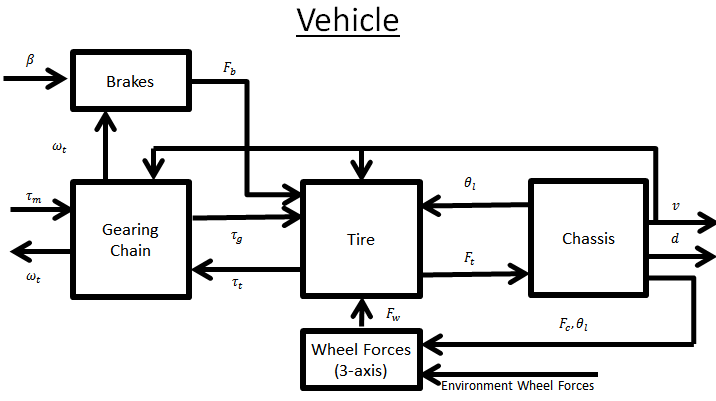
\includegraphics[scale=.75]{Vehicle_Diagram}
  \caption{Vehicle Diagram}
\end{figure}

\subparagraph{Gearing/Chain}

\begin{gather}
\dot{\omega_t} = \frac{\tau_m - \tau_t}{J_m + J_g + J_t} \\
\tau_g = \frac{\tau_m \eta (\omega_t)}{R_g}
\end{gather}

\subparagraph{Brakes}

\begin{gather}
F_b = \mu_b w_t \beta
\end{gather}

\subparagraph{Tire}

\begin{gather}
\kappa_t = 
\left\{
  \begin{array}{lr}
    0.0085 + \frac{0.18}{p_t} + \frac{1.59*10^{-6}}{p_t} & : v_{kph} \le 165 (km/h)\\
    \frac{0.18}{p_t} + \frac{2.91*10^{-6}}{p_t} & : v_{kph} > 165 (km/h)
  \end{array}
\right. \\
\tau_t = \tau_g - \frac{F_{w,long}}{r_t} - \frac{F_b}{r_b} - \kappa_t F_{w,n} v_{kph}^2 \\
F_{max} = m_{t,gnd} F_{w,n} \\
F = \tau r_t \\
F_t =
\left\{
  \begin{array}{lr}
	F & : -F_{max} \le F \ge F_{max} \\
	F_{max} & : -F_{max} < F or F > F_{max}
  \end{array}
\right. \\
\lambda = \frac{v - \omega_t r_t}{v}
\end{gather}

The piece-wise function associated with $F_t$ is an attempt to follow the curve below.

 \begin{figure}[H]
  \centering
  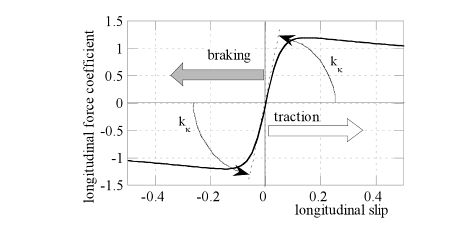
\includegraphics[scale=1]{wheel_slip}
  \caption{Force Coefficient Curve}
\end{figure}

\subparagraph{Wheel Forces}

\begin{gather}
F_{\omega,long} = F_{c,long} \\
F_{\omega,n} = F_{c,n}
\end{gather}


\subparagraph{Chassis}

\begin{gather}
F_a = \frac{1}{2}\rho(d)C_dAv^2 \\
F_{c,long}  = F_a + gm\sin(\theta_r (d))  \\
F_{c,n} = mg\cos(\theta_r (d)) \\
\dot{v} = mF_t
\end{gather}

\subparagraph{Environment}

\begin{gather}
given: alt(d) \\
\theta_r  = \frac{d}{dd} alt(d) \\
T_amb(d) = T_0 - L alt(d) \\
P(d) = P_0 \left( 1 - \frac{L alt(d)}{T_0} \right)^{\frac{gM}{RL}}\\
\rho(d) = \frac{PM}{1000RT}  
\end{gather}


\end{document}


\begin{figure}[H]
  \centering
  \includegraphics[scale=0.25]{p1_b}
  \caption{Coefficient of Variation of IMEP per Cylinder}
\end{figure}

